\chapter{EXPERIMENTAL ASPECT}

\section{Relativistic Heavy Ion Collider (RHIC)}
This dissertation is a part of research conducted at the relativistic heavy ion collider (RHIC) at Brookhaven National Lab (BNL), located at Upton, New York, United States. RHIC is the world's first collider, which can collide polarized proton beams up to center-of-mass energy of $\sqrt{s} =$ 510 GeV. It can also collide heavy ion particles of varying energy up to $\sqrt{s} =$ 200 GeV. The detailed overview of the RHIC complex and its components are discussed in reference \cite{Alekseev:2003sk}. Relevant components of the RHIC that have a direct impact on this analysis are discussed in this section.   

\drawgraphics{1}{ExperimentalAspect/Rhic\_complex.png}{Relativistic heavy ion collider complex \cite{rhic}.}{fig:rhic}
   
\subsection{Siberian Snakes and Spin Dynamics}
\label{subsec:snakes}
In high-energy particle colliders, it is important to understand the evolution of the spin of the highly accelerated colliding beam and the tools that control it.  
For a circular accelerator as RHIC, the spin evolution in the external magnetic field is given by the Thomas-BMT equation \cite{Thomas:1927yu, Bargmann:1959gz},
\begin{equation}
    \frac{d\vec{P}}{dt} = -(\frac{e}{\gamma m})[G\gamma \vec{B}_\perp + (1+G)\vec{B}_\parallel]\times \vec{P},
\end{equation}
where $\vec{P}$ is the polarization vector expressed in the frame that moves with the particle. $G(=1.7928)$ is the anomalous magnetic moment of the proton and $\gamma = E/m$. $G\gamma$ is called the spin tune $\nu_{sp}$, which gives the number of full spin precessions in every full revolution. The value of the $\nu_{sp}$ can reach up to 478 at the RHIC top beam energy of 250 GeV. 

It isn't easy to maintain the polarization of the highly accelerated beam in the circular path. Two resonances cause the depolarization; one is due to the misalignment and magnet errors called ``imperfection resonances", and the other is called ``intrinsic resonances," caused by the focusing magnetic fields. The imperfection resonances occur when $\nu_{sp}=G\gamma = n$, where $n$  is an integer. In contrast, the intrinsic resonance occurs when $\nu_{sp} = G\gamma = kP \pm \nu_y$, where $k$ is an integer, $\nu_y$ is the vertical betatron tune, and $P$ is the superperiodicity. These resonances cause the spin of the polarized beam to be fully flipped (slowly accelerated beam) or partially flipped (highly accelerated beam), which are traditionally overcome using a betatron jump. At RHIC, ``Siberian Snake" is used to maintain the stable beam polarization, which can produce a 180\textdegree \ spin rotation about the horizontal axis, which is greater than the spin rotation due to the depolarization resonances. These Siberian snakes are constructed either by using a solenoidal magnet or a sequence of interleaved horizontal and vertical dipole magnets producing local orbit distortion. A full snake is used; however, for a low-energy accelerator, a partial snake suffices to maintain stable beam polarization overcoming the depolarization resonances. 

\subsection{Polarized Proton Injector}
The RHIC polarized beam requires a bunch intensity of $2\times 10^{11}$ protons per bunch. To meet this requirement, the alternating gradient synchrotron (AGS) needs to reach bunch intensity of $4\times 10^{11}$ to allow room for some losses while transferring it to the RHIC rings. The optically pumped polarized ion source (OPPIS) produces a polarized $H^-$. It produces 500 $\mu A$ in a single  300 $\mu s$ pulse, which corresponds to the $9\times 10^{11}$ polarized $H^-$. The polarized $H^-$ ions are accelerated to 200 MeV with a radio frequency quadruple (RFQ) and 200 MHz LINAC with an efficiency of about 50\%. The pulse of $H^-$ ions is strip-injected and captured in the AGS Booster as a single bunch, containing $4\times 10^{11}$ polarized protons. Each polarized proton bunch is accelerated to the Booster to 1.5 GeV kinetic energy and transferred to the AGS, which is accelerated to 25 GeV. Finally, the beam bunches are handed to the RHIC rings for further acceleration to 100 or 250 GeV.     


\subsection{Acceleration in the Booster and the AGS}
The polarized proton bunch in the AGS may lose its polarization due to the  depolarization resonances. This is overcome by installing a partial (5\%) Siberian snake at one of the straight sections of the AGS, which is sufficient to avoid any depolarization due to imperfection resonances. The acceleration and beam transfer efficiency is greater than 50\%, giving $2\times 10^{11}$ protons per bunch. This process is repeated until all 120 bunches of the RHIC ring are filled. 

\subsection{RHIC Rings General Layout}
Two full Siberian Snakes on the opposite side of each RHIC ring opposite side serve to avoid depolarization from imperfection and intrinsic depolarization resonances up to the top energy of 250 GeV. These Siberian Snakes introduce a 180\textdegree\ spin rotation around the horizontal axis  without generating a net orbit distortion. In addition, the two axes of the two Snakes in each ring must be perpendicular. Moreover, Snakes are installed in the exact opposite direction in the ring; in fact, the beam direction in one snake should be exactly opposite. Two pairs of Snakes, one pair in each ring, are installed at the 3 and 9 o'clock sections of the RHIC as shown in figure \ref{fig:rhic}.

To achieve the desired beam polarization at the interaction region, a set of two pairs of spin rotators, two sets of that one for the STAR and the other for the PHINIX, are installed right before and after the interaction region. The equilibrium position of the beam polarization is the transverse direction. Whenever a longitudinal polarization is needed, the spin rotators before the interaction rotates the beam polarization to the longitudinal direction, and the rotators beyond the interaction point bring it back to the transverse direction. Having its own set of spin rotators for the STAR and PHENIX experiments allowed an independent choice of beam polarization simultaneously.   

\subsection{Polarimetry}
Measuring the beam polarization with higher precision at RHIC is crucial, as the polarization value normalizes many spin physics analyses. There are two proton-carbon (pC) Coulomb Nuclear Interference (CNI) \cite{KURITA2003C356}, one in each ring, for the relative polarization measurement, and one hydrogen gas jet (H-jet) polarimeter \cite{Zelenski:2005mz} at one of the interaction points for the absolute polarization. 

The pC CNI polarimeter uses a very thin ribbon of carbon targets developed by IUCF, which is simpler and easy to handle in the vacuum than the H-jet CNI. The analyzing power of pC CNI is about 3-5\% for an elastic scattering in the small angle CNI region with a larger cross section being weakly energy dependent over the RHIC energy range from 24 GeV/$c$ to 250 GeV/$c$—the carbon target results in the high luminosity required for fast polarization measurements. The sizeable analyzing power, larger cross section, and the advantages of the solid carbon target make this process ideal for a fast primary RHIC polarimetry.   

The H-jet CNI polarimeter is located at the IP-12 in the RHIC ring, which is close to the pC CNI polarimeter, as shown in figure \ref{fig:rhic}. It is used for the absolute polarization measurement based on the elastic $pp$ scattering in the CNI region. It consists of three parts: the polarized atomic beam source (ABS), the scattering chamber, and the Breit-Rabi polarimeter \cite{Baumgarten2002}. With the state-of-art of ABS, the thickness of the H-jet target is $\sim 10^{12}$ atoms/$cm^2$. The  polarimeter target is free from the atomic beam, which crosses the RHIC beam in the vertical direction. Because of the particle identity, the beam polarization can be directly expressed in terms of the proton target polarization, which is directly measured by the Briet-Rabi polarimeter. Since it is remotely located, there is minimal interference with the other experiments, and it excludes the background generations for the other experiments.   

\section{STAR Detector and Sub-Systems}
The solenoidal tracker at RHIC (STAR) is one of the two large detectors constructed at the six o'clock position in the RHIC complex at Brookhaven National Laboratory (BNL). It is constructed to investigate the behavior of strongly interacting matter at high energy density and to search for the signatures of quark-gluon plasma formation. Moreover, the polarized proton-proton collision program opened up multiple opportunities for the spin physics study of the quarks and gluon in a proton. STAR can measure a hadron production over a large solid angle, featuring detector systems for high-precision tracking, momentum analysis, and particle identification. In addition, large acceptance of the STAR allows event-by-event characterizations of heavy ion collisions and detection of a hadron in jets.

\drawgraphics{0.8}{ExperimentalAspect/STARdet.jpg}{Perspective view of the STAR detector, with a cutaway for viewing inner detector systems.}{fig:stardet}


\drawgraphics{1}{ExperimentalAspect/StarDetCutaway.jpg}{Cutaway side view of the STAR detector \cite{Sakuma2010}.}{fig:starcs}

Figure \ref{fig:stardet} displays the STAR detector layout with a cutaway revealing the inner detector systems. The STAR detector system, cylindrical in shape, includes multiple detectors working in unison. The interaction point is at the center of the detector system, where the closest detector to it is the Silicon Vertex Tracker (SVT) \cite{STAR:2002bzu}. The SVT spans $|\eta|\leq 1$ in pseudorapidity with full azimuthal coverage ($\delta\phi=2\pi$), which provides charged particle tracking, precision localization of the primary vertex, and identification of secondary vertices from the weak decays, for example, $\lambda$, $\Xi$, and $\Omega$s. The Time Projection Chamber \cite{Anderson:2003ur}, which is the heart of the STAR detector system, provides charged particle tracking, Particle Identification (PID), and momentum reconstruction using a 0.5T field from the solenoidal magnet \cite{STAR:1992kiw}. The details of the TPC are discussed in section \ref{subsec:tpc}. The charge particle tracking in the forward region is provided by the Forward TPC (FTPC) \cite{Ackermann:2002yx}, which has a coverage of $2.5 <\eta < 4$ in pseudorapidity with complete azimuthal coverage and symmetry. Moreover, the PID capability of the STAR is extended in the central region ($|\eta|<0.3$) by installing the ring imaging Cherenkov (RICH) detector \cite{STAR:2002aln}. The RICH provides PID of pions and kaons up to $\sim 3$ GeV/$c$, and that for protons up to $\sim 5$ GeV/$c$. In addition, a Time of Flight (TOF) \cite{STAR:tof} detector vastly improves STAR PID by providing the timing information with the same coverage as the TPC in $\eta$ and $\phi$, which is discussed in section \ref{subsec:tof}.    
The STAR event triggering system is based on the transverse energy of the events measured by the electromagnetic calorimeter in the barrel region (BEMC) \cite{STAR:2002ymp} and in the endcap region  (EEMC)\cite{STAR:2002eml}. The BEMC and EEMC have a $-1<\eta<2$ coverage in pseudorapidity and whole $2\pi$ azimuthal angle.


\subsection{TPC and Magnet}
\label{subsec:tpc}
Figure \ref{fig:tpc} shows the schematic view of the STAR TPC. It's cylindrical, measuring 4 meters long and 4.2 meters in diameter. Its acceptance covers $|\eta|\leq 1.8$ in pseudorapidity and full $2\pi$ coverage in azimuth over a full range of multiplicities, which makes it one of the largest operating TPC in the world. It sits in a large solenoidal magnet that operates in a 0.5 T magnetic field. It consists of a thin conductive Central Membrane (CM) at its center, which is 70 $\mu$m thick carbon-loaded Kapton film with a surface resistance of 250 \si{\ohm} per square that operates at 28 kV potential, with the end caps at the ground  providing a uniform electric field of 135 V/cm. The proper boundary conditions between the CM, end caps, and field cage cylinders establish the uniformity of the electric field. The field cage cylinders, inner field cage, and outer field cage, shown in figure \ref{fig:tpc}, provide a series of equipotential rings that divides the space between the CM and the anode planes into 182 equally spaced segments. One ring is common to both sides, where the CM sits. The uniform gradient between the CM and the grounded end caps is maintained by biasing these rings with a chain of precision resistors  of 2 M\si{\ohm}.

   \drawgraphics{1}{ExperimentalAspect/StarTPC.eps}{STAR time projection chamber.}{fig:tpc}

The empty volume between the field cages is filled by the P10 gas, which is 10\% methane and 90\% argon at 2 mbar coverage above atmospheric pressure \cite{Kotchenda:2002rqz}. The P10 gas attributes the fast drift velocity, peaking at a low electric field, which provides the stable drift velocity of the particles insensitive to the variation in the atmospheric conditions, temperature, and pressure.  

The STAR experiment uses the TPC as the primary tracking device, which records particle tracks, measures particle momenta, and identifies the particles by measuring their ionization energy loss ($dE/dx$). It effectively separates pions and protons up to 1.2 GeV/c; however, separating high-energy particles is difficult as the dE/dx becomes less mass dependent at higher energies. As the primary ionizing particles enter the TPC gas volume, their paths are reconstructed with high precision from the released secondary electrons, which drift in the electric field to the readout end caps at the end of the chamber. The TPC performance relies heavily on the magnetic field as electrons may diffuse in the transverse direction, directly impacting particle track reconstruction. The momentum resolution for most of the tracks in the TPC reaches the value of $\delta p/p = 0.02$. The relative momentum resolution increases for a low-momentum track with more hits points along the track. 

The electric and magnetic fields in TPC are uniform all around, radially as well as longitudinally. However, the non-uniformities and global misalignment of the electric and magnetic fields can cause distortions in the position of the secondary electrons reaching the readout pads. One of the causes of the field distortion in TPC is the space charge which occurs due to the piling-up of slow drifting positively charged ions in the gas from the standard operation of the TPC \cite{VanBuren:2005qg}. The effect is propagated to the recorded tracks, corrected by the well-established space charge and grid leak calibration procedure. 

\subsection{Barrel Electromagnetic Calorimeter (BEMC)}
\label{subsec:bemc}
The schematic view of the Barrel Electromagnetic Calorimeter (BEMC)\cite{STAR:2002ymp} is shown in figures \ref{fig:bemcxsec} (cross section view) and \ref{fig:bemcside} (side view). The BEMC sits underneath the aluminum coil of the solenoid covering the $|\eta|\leq 1$ and $2\pi$ in azimuth at a radial distance of about 220 cm from the beam axis matching the coverage of the TPC acceptance. 

\begin{figure}
\begin{subfigure}{0.8\textwidth}
\centering     
    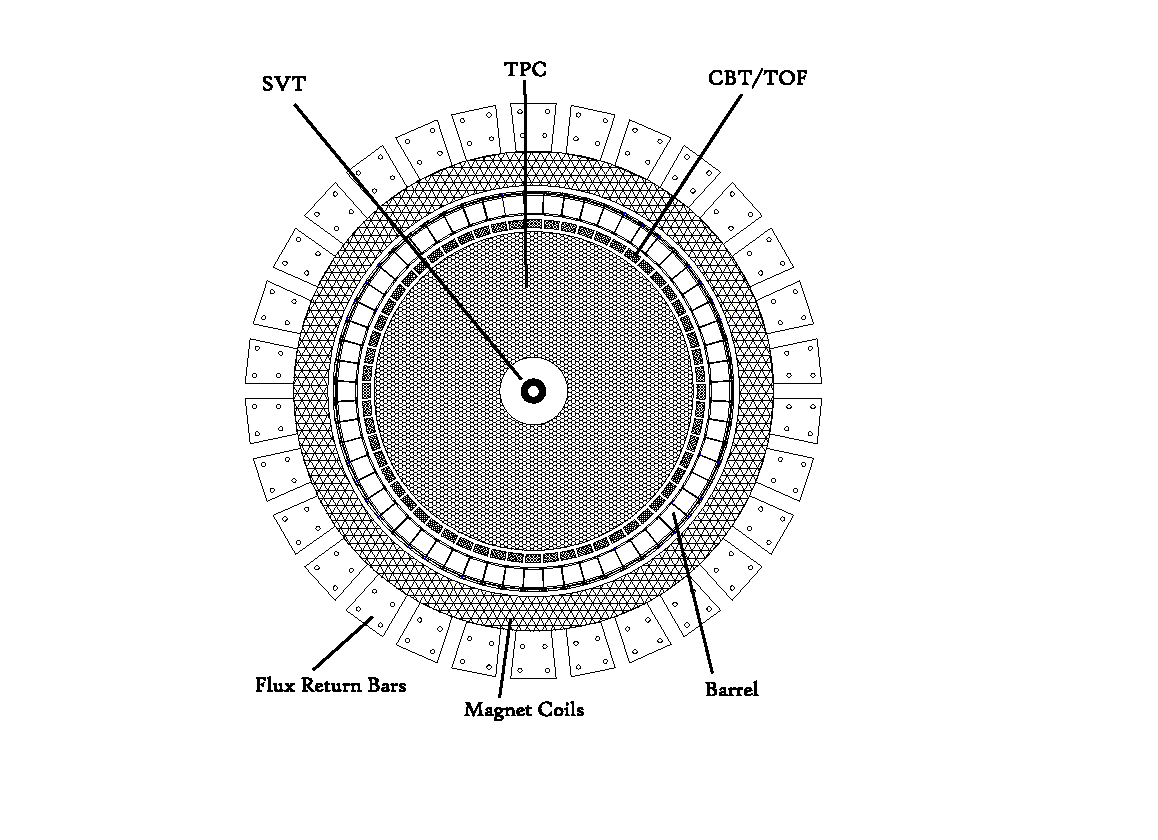
\includegraphics[scale=0.8]{ExperimentalAspect/BEMC_cs.eps}
    \subcaption{BEMC Cross Section view}
    \label{fig:bemcxsec}    
\end{subfigure}
\begin{subfigure}{0.8\textwidth}
\centering
    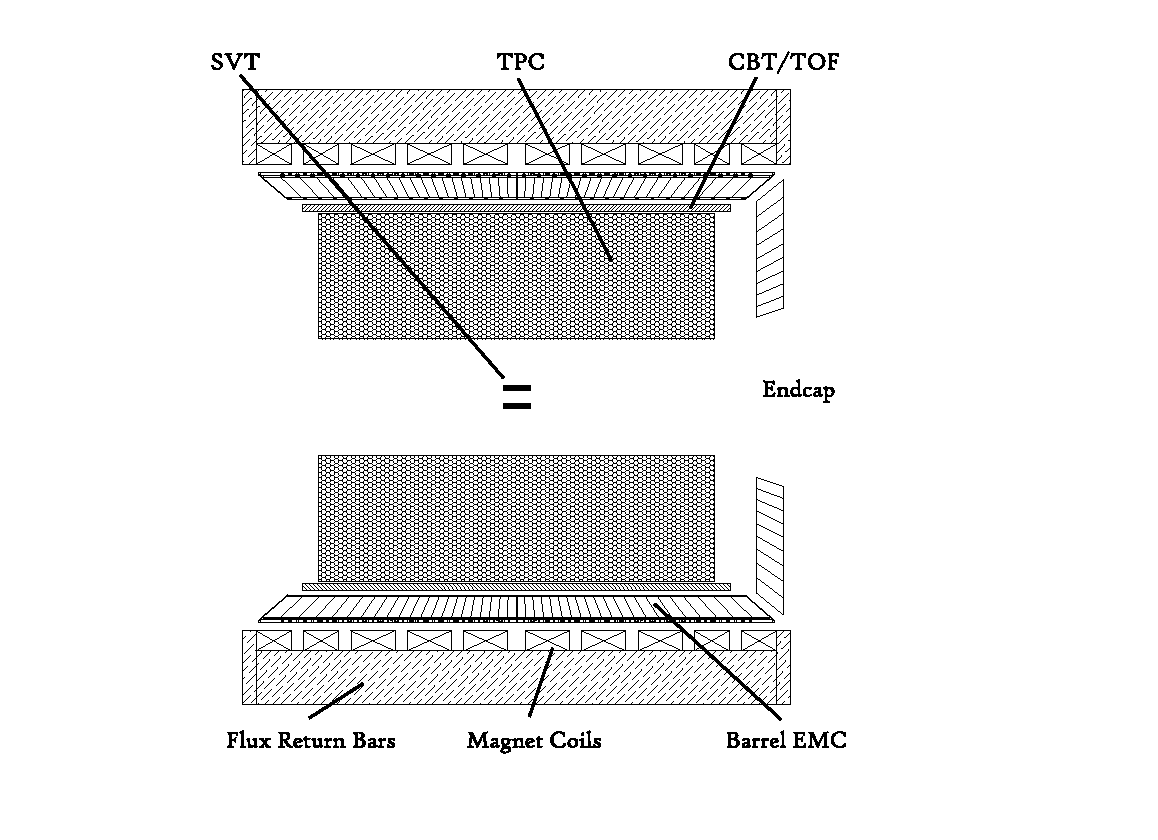
\includegraphics[scale=0.8]{ExperimentalAspect/BEMC_side.eps}
    \subcaption{BEMC Side view}
    \label{fig:bemcside}
 \end{subfigure}
 
\end{figure}
The BEMC design includes 120 calorimeter modules placed 60 in $\phi$ and 2 in $\eta$. Each module measures about 26 cm wide and 293 cm long with an active depth of 23.5 cm, each subtending 6\textdegree\  in $\Delta \phi$ and 1 unit in $\Delta\eta$. Each module is divided into 40 towers, 20 in $\eta$ and 2 in $\phi$, with each tower subtending 0.05$\times$0.05 in $\Delta\phi \times \Delta\eta$.  Thus, the BEMC comprises 4800 calorimeter towers spanning a full $2\pi$ coverage in azimuth. Each of the towers is constructed so that they point to the interaction diamond at the center. This projective nature of the tower in a module is shown in figure \ref{fig:bemcproj}.

\drawgraphics{1}{ExperimentalAspect/BEMC_sideprojective.eps}{Side view of the BEMC module.}{fig:bemcproj}

The core of the calorimeter consists of a stacked layer of 5 mm thick lead and 5 mm plastic scintillator alternately and a Shower Max Detector (SMD) situated roughly at five radiation lengths from the front of the stack. There are 21 active scintillating layers and 20 layers of lead absorber plates. The plastic scintillator, called ``megatile", consists of 40 optically isolated tiles. The mechanical structure of a calorimeter module with the compression components and the rail mounting system is shown in figure \ref{fig:bemcmoduleside}.
 
\subsection{Time of Flight (TOF)}
\label{subsec:tof}
The STAR Time of Flight (TOF) compliments the particle identification capability of the TPC by using the timing information in conjunction with the vertex position detector (VPD). TOF sits outside the TPC, wrapping all around and spanning the same coverage as the TPC. The TOF system is designed based on the multi-gap resistive plate chamber (MRPC), first developed by the CERN ALICE group \cite{Williams:2001mt}. The side view of the MRPC module for the STAR TOF system is shown in Figure \ref{fig:tofmodule}. The long edge of the module is shown at the top, whereas the bottom figure shows the short edge. The MRPC module consists of a series of  0.54 mm thick glass plates kept parallel by using 0.22 mm diameter nylon fishing line as a spacer. A mixture of 90\% C2H2F4, 5\% isobutane, and 5\% SF6 fills the gaps between the plates. The resistivity of these glass plates is of the order of $10^{13}$ \si{\ohm}/cm, thus being transparent to the electrical charges. These plates are electrically floating, and a strong electric field is generated in each sub-gap of gas with the electrodes applied on the outer surface of the outer plate. Since the glass plates and electrodes are charge transparent, the induced signal picked up by the copper readout pad is the sum of all the avalanche of charges induced in the gas gaps.  

The TOF system measures time intervals for a particle track using two detectors; one is the VPD (see section \ref{subsec:vpd} for details), which provides an event start time, and the TOF MRPC provide the stop time for reconstructed charged tracks that point back to the event vertex. This time interval, $\Delta t$, for reconstructed tracks, with the momentum, $p$, and total path length, $s$, allows us to calculate the inverse velocity, $1/\beta$, for each track as, 
\begin{equation}
    \frac{1}{\beta}  = \frac{c\Delta t}{s},
\end{equation}
where $c$ is the speed of light. With $1/\beta$ and $p$, the particle mass, $m$, can be calculated as,
\begin{equation}
    m = p \sqrt{1/\beta^2 -1}
\end{equation}

$\beta$, as calculated above using the TOF system timing information, versus particle momentum provides a basis for the TOF particle identification. 

In recent studies, it has been observed that for an event vertex with the z-vertex position difference identified by the TPC  ($V_{z,tpc}$) and VPD ($V_{z,vpd}$) greater 5 cm, the VPD timing information may be incorrect. 
A new method was developed called ``StartLessTOF", which addresses this issue by calculating the start time starting at the stop time and moving backward for a track without relying on the VPD timing. In the IFF asymmetry analysis, discussed in chapter \ref{chapter:iff}, the StartLessTOF method of PID is used, and more details will be discussed in the respective section.  

\drawgraphics{0.9}{./ExperimentalAspect/TOFmodule.jpg}{Side view of an MRPC module for the long (top) and short (bottom) sides.}{fig:tofmodule}

\subsection{Vertex Position Detector (VPD)}
\label{subsec:vpd}
There are two identical Vertex Position Detector (VPD) \cite{Llope:2014nva} assemblies, one at the east side and the other at the west side, located symmetrically surrounding the beam pipe at a distance of 5.7 m from the TPC center. Each VPD assembly consists of nineteen detectors, each composed of a lead (Pb) converter followed by a plastic scintillator read out by a photo-multiplier tube. The side view of this detector assembly is shown in figure \ref{fig:vpdside}. The front view of the VPD with all nineteen detectors assembled in two circles is shown in figure \ref{fig:vpdfront}.  

\drawgraphics{0.8}{./ExperimentalAspect/VPDfrontview.png}{VPD front view.}{fig:vpdfront}

\drawgraphics{0.8}{./ExperimentalAspect/VPDsideview.png}{VPD side view.}{fig:vpdside}

The VPD can provide timing information of an event, which is required for event triggering and for a fast detector as the event start time, for example, TOF. It measures the vertex $z-$position. It provides the timing information by measuring photon arrival time produced by the decay of $\pi^0$ in the very forward direction, close to the beam pipe.   

Besides serving as the primary detector input for the minimum bias trigger in A+A collisions, each VPD assembly measures up to nineteen times in each event, which is used to measure the location of the vertex along the beam direction, $Z_{vtx}$, given by,
\begin{equation}
    Z_{vtx} = c(T_{east} - T_{west})/2,
    \label{eq:vzvpd}
\end{equation}
where $T_{east}$ and $T_{west}$ are the times measured by the two VPD assemblies. Moreover, the start time used by the TOF for the particle identification, $T_{start}$ is given by, 
\begin{equation}
    T_{start} = (T_{east} + T_{west})/2 - L/c,
\end{equation}
where L is the distance of either assembly from the center of the STAR. The experimental resolution of the VPD timing, $T_{east}$ or $T_{west}$, depends on the number of channels used in the assembly $N$, which improves as $\delta T \propto 1/\sqrt{N}$, where $T$ is $T_{east} $ or $T_{west}$. Which follows the $Z_{vtx}$ resolution of equation \ref{eq:vzvpd} given by, 
\begin{equation}
    \delta Z_{vtx} =(c/2)\delta \Delta T = (c/\sqrt{2})\sigma_0 /\sqrt{N},
\end{equation}
where $\sigma_0$ is the time resolution of the single readout detector and $\delta \Delta T$ is the resolution of the time difference ($T_{east} - T_{west}$). Thus, the large number of readout channels allows averaging over more lit channels, improving the overall VPD performance.  


 